\chapter{Related work}

I will use this chapter to provide an insight into the world of \emph{agents} and spatial memory. I hope you will not be disappointed as you will not find \textit{007} in the following lines.

\section{Agents}

There are several ways to explain what or who an \emph{agent} is. Apart from systems of agents used in philosophy or sociology, we can see a first modern use of agency and agents in economy where economists have substituted a human with a simpler agent. They intended to simplify their economic models in order to carry out general simulations. Buyers and sellers are typical examples of agents used in simplified market model in microeconomics. In this context, agents are entities in the model which can react to a given context.

In the case of artificial intelligence, we can use the definition of an agent found in \cite{russel2003ai}. It could not be simpler:

\begin{definition}{\bf Agent} is just something that acts.
\end{definition} 

Of course it is as general as it could be and for our purposes this is too simple, so we will use another definition which meets better the context of this work.

\begin{definition}{\bf Agent} is something that senses the environment and affects it using its actuators.
\end{definition} 

As a further source on the topic of intelligent agents see \ref{Wooldridge:intelligentagents}.

Having defined an agent, we can now begin to distinguish specific kinds of agents. In this thesis I will use several slightly different terms in order to refer to agents: \emph{rational, autonomous, plausible and believable}. 

A \emph{rational agent} refers back to economics, where we can find a definition of rational behaviour. Even though it is rather a hypothetical model since people are usually irrational in their decisions from the perspective of economics, the definition used in economics suits our needs well. A rational agent is one that acts as if balancing costs against benefits to arrive at action that maximizes personal utility (Milton Friedman (1953), Essays in Positive Economics). In simple terms, the agent does what is or perhaps might be the best for him based on his current knowledge of the world.
 
Rational behaviour might, however, be understood in a completely different way. \emph{Plausible agents} are agents where the basic approach is to implement human-like internal processes. A well-known example is that of neural networks, although these are usually used in a simplified way. Since it is really difficult to implement a completely plausible agent, there are many research teams focusing on specific parts of the complex human nature.

\emph{Believable agents} are personality-rich autonomous agents with the powerful properties of characters from the arts \cite{Loyall:believableagents}. 

The last type of agents is referred to as autonomous. An \emph{autonomous agents} are able to accomplish a useful task or are effective problem solvers.

One additional term should be defined in reference to agents:

\textit{Belief-Desire-Intention (BDI) agency model} implements three parts: agent's belief, his desire and his intention. These three parts are combined in reasoning. A BDI agent is a particular part of a \textbf{bounded rational agent}, which uses the three parts to separately prepare plans which are later executed. What distinguishes BDI from a simple reactive agent is that a reactive agent creates an immediate decision based on the current state of environment and the inputs of his sensors. The BDI agent, on the hand, uses all three parts:

\begin{itemize}
\item {\bf belief} represents the agent's informational state, for example sensory inputs and information in his memory,
\item {\bf desire} is the agent's motivational state, what he needs to approach, for example he is hungry and he needs to find appropriate food,
\item {\bf intention}, on the other hand, is his immediate decision how he attaing the goal he desires, in other words it is execution of plan, for example next move.
\end{itemize}

\section{Spatial resource-bounded memory}

A memory is something that changes a reactive agent into an agent with an ability to learn. It can be used for learning consequences of agent's acts, conditional dependencies in the agent's world (citation for Bayesian networks), or spatial information about the environment. The latter is a kind of memory we used for agents in our simulation. 

A spatial memory is used when the agent needs to navigate usually in a two or three dimensional space. In short, it is a component of the agent which tells him where to go when he needs or wants to do something. There are several different approaches and several examples are going to be covered in this section. I am going to introduce several existing implementations of spatial memory. Mainly I will attempt to address whether and how they have dealt with bounded resources - either due to implementation restrictions, or when approaching plausibility in their models.

\subsection{Resource-bounded reasoning}

Rational agents cannot be expected to be able to compute a load of data in a constant time or in a time in which the environment doesn't change much. That is why we have to take into account bounded resources when simulating plausible or real agents. What we want to avoid is the computation of plan that takes a long period of time during which the environment changes significantly. As noted by Bratman \textit{et al.}, plan computation can be separated from plan execution, whereby the plan is prepared over several executions. \cite{Bratman:practicalreasoning} In this case we need either to be able to perfectly predict the future, or base our plan on data, which does not change at all or remains constant for the given period of time.

\subsection{Short-term and long-term memories}

Generally, when we talk about remembering something, two terms need to be defined: a long-term memory (LTM) and a short-term memory (STM). Both of these describe a capacity for holding a certain amount of information in mind. Apart from the varying amount of information stored, the memories differ in the availability of such information and the period of time over which these memories last.      

In 1968 Richard Atkinson and Richard Shiffrin suggested a memory model divided into three components \cite{Atkinson:humanmemory}: 

\begin{enumerate}[(a)]
\item \emph{sensory register}, able to store only a relatively small amount of data for a short period of time,
\item \emph{short-term store} with the ability to store also a limited amount of data, but for a longer period of time,
\item \emph{long-term store} with a large capacity for a nearly unlimited amount of time.
\end{enumerate}

\begin{figure}
  \centering                                
  \includegraphics[scale=0.5]{diagrams/usedalgorithms/atkinson-memory.eps}    
  \caption{Information flow in the memory system, adopted from Atkinson \textit{et al.} \cite{Atkinson:controlofrtm}}
  \label{usedalgorithms:qttv}
\end{figure}

We use {\bf short-term memory} to store information for a relatively short period of time. This could be seconds or minutes. A number of entites we are able to hold in the STM was studied by George Miller in 1956. \cite{Sternberg:congitivepsychology} The outcome of his work was the magical number $7\pm 2$, which is the number of similarly small things we can hold in STM.

A \textbf{long-term memory}, on the other hand, is used to store information we do not think of consciously. The pieces of such information are important for the everyday life. The capacity of LTM memory is unknown, as there is no way how to measure it. 
                                               
\subsection{Computational memory architectures}

Computational memory architectures for autobiographic agents interacting in complex virtual environment suggested by Ho \textit{et al.} work with both short-term and long-term autobigraphic memories, where they have studied the agent’s ability to survive in comparison to a purely reactive agency model. \cite{Ho:memoryarchitectures} Moreover, they researched whether the narrative communication amongst agents somehow positively influence those agents. They have separately experimented with three types of agents: purely reactive (PR), short-term memory (STM) and long-term memory (LTM). A purely reactive agent walks randomly around the environment avoiding obstacles and searching for resources in order to to fulfil his needs.

STM agents in further extend the model of purely reactive agents and add a track-back memory system in addition to the reactive behaviour. Each time an agent deals with an event (e.g. collision, or resource object), he confines this information into his memory. They refer to this as an event-based memory entry making mode. These events are kept in a linear list of a finite size and the oldest events are deleted. The memory is used when an internal variable is over threshold. That is the moment when agent searches in his memory for an information about relevant resource object. If he succeeds, he retrospectively undoes all memorized states leading to the relevant one (\textbf{nechapu)}. Therefore, what the STM agents (\textbf{kdo je they????)} actually store in memory is an agent’s current state: where he has been and what he has perceived. While attaining imperfection (\textbf{attaining? nerozumim)} in retrieving information from short-term memory, they introduced noise distortion using Gaussians \textbf{(noise distortion? ne reduction nebo tak neco?)}.

LTM is mostly based on psychological autobiographic memory models. There are three parts that are involved in the reasoning process: Event Specific Knowledge (ESK), Event Reconstruction Process (ER) and Event Filtering and Ranking Process.

\textbf{DOPLNIT JEJICH ZAVERY}

\subsection{How Place and Objects Combine?}
\label{subsec:howplaceandobjectscombine}

Brom \textit{et al.} mainly focused on plausible behaviours while searching for things in structured spaces such as flats.\cite{Brom:placeandobjects} Unlike others who previously researched the area of spatial memory for plausible agents, they suggested a model for an agent which could successfully live in a dynamic environment with objects that could be moved without the agent’s involvement. 

In this model, the environment consists of abstract and specific areas such as rooms and pieces of furniture. These areas are combined into a tree structure used in the model where, for example, the flat is a root node, the immediate child nodes are rooms and, finally, specific pieces of furniture are child nodes below room nodes. Four different categories have been created for objects to reflect varying probabilities of changing object’s location which in fact simulates a presence of another agent in the environment. The observed agent therefore does not leave the flat and it is there alone.

During their experiments, what is interesting for my work is the subsequently observed ability of the model to emerge (\textbf{nechapu emerge}) the searching rules from scratch, to relearn the rules in the case a particular setting changes, \textbf{and if the merged rules meet with the human behaviour, i.e. they are believable. (nedava smysl)}
                 
\subsection{Inspirations for my work}

The suggested RTM and LTM models of agents as described by Ho et al. are of interest in my simulation. \cite{Ho:memoryarchitectures} There has to be a couple of minor changes, though, as I am working with a simpler environment compared to the one used in the work described above. The changes will influence the structure of memory records in both RTM and LTM. Also the communication protocol will be different and I am going to introduce it later in this thesis. Although it is not going to be part of this particular thesis, comparing the memory models might prove interesting.

In my project, the environment I want to use does not differentiate the area as the one assumed by Brom \textit{et al.}, that means it is homogeneous. \cite{Brom:placeandobjects} For the purpose of implementing an agent with a similar spatial "What-where" memory model, I will use a different spatial organization, which could be similarly structured into a grid. The suggested model, however, is usable for objects which are moved around the environment and I do not have such objects. Objects in my environment are generated around a distribution place and locations of those places are something that could be learnt using “What-Where” model. 